\documentclass[10pt, a4paper]{article}
\usepackage[utf8]{inputenc}
\usepackage{fullpage}
\usepackage{array,url,kantlipsum}
\usepackage{amsmath}
\usepackage{amssymb}
\usepackage{array}
\usepackage{color}
\usepackage{wrapfig}
\usepackage{tabu}
\usepackage[labelfont=bf]{caption}
\usepackage[font={small}]{caption}
\usepackage[explicit]{titlesec}
\usepackage{graphicx}
\usepackage{gensymb}
\usepackage{pgfgantt}
\usepackage{textcomp}
\usepackage{perpage}
\usepackage{color,soul}
\usepackage{subfig}

\graphicspath{ {Images/} }


\usepackage{verbatim}

\title{backgrounds_report}
\author{Oliver Hall}
\date{January 2018}

\newcommand{\HRule}{\rule{\linewidth}{0.3mm}} 


\begin{document}

\titlepage

\tableofcontents
\pagebreak

\section{Introduction}
This quick report breaks down the individual background estimators for TESS Full Frame Image s(FFI) on the TASOC/SkyBackgrounds repository and gives a visual guide to how they fare against increasingly complex backgrounds.

\subsection{CvE esitmate}
The CvE estimate (method author: Carolina van Essen) attempts to find the background continuum along each row in the FFI and consequently each column, after which these are averaged together.\\

This is done by binning each column/row of data, finding the value of a user-chosen percentile (default: 10) in each bin, and smoothing across these values to find the background continuum. See Figure \ref{fig:cve} for an example on a single row in Y.\\

Pros:
\begin{itemize}
\item Very fast
\item Works well when approriate percentile is chosen
\end{itemize}

Cons:
\begin{itemize}
\item Percentile must be chosen by the user (supervised)
\item Background has artificial small scale structure due to seperate binning in X and Y
\end{itemize}

\begin{figure}[h!]
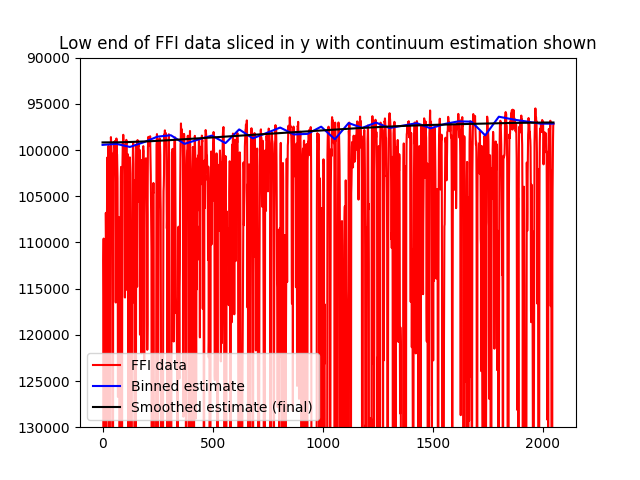
\includegraphics[width=\textwidth]{CvE_example}
\caption{Example of CvE run on the first row in Y for a TESS FFI.}
\label{fig:cve}
\end{figure}

\subsection{ML estimate}
The ML method (method author: Mikkel Lund) attempts to fit to the background continuum by first finding the mode of subsections of the full FFI and fitting to these.\\

First, the data is subdivided into squares of a given width and height (default: 128 pixels). Then we run RANSAC to fit to the continuum of the data in each of these squares, producing an inlier mask. The mode is taken as the location of the maximum value of a Kernel Density Estimate (KDE) on the data considered by RANSAC to be an inlier to the continuum (this eliminates high flux pixels containing stars). These modes are then again fit to using RASAC to obtain inlier masks, which are then used as weighting factors for a subsequent polynomial fit of a user-selected order.\\

Pros:
\begin{itemize}
\item Achieves good results when appropriate polynomial order is chosen.
\item Mode calculation is very accurate
\item Running on multiple FFI frames allows for re-use of RANSAC inlier masks.
\end{itemize}

Cons:
\begin{itemize}
\item Require input of the correct polynomial order (supervised)
\item Runs very slowly for a single FFI
\item Polynomial fitting eliminates small scale structure
\end{itemize}

\subsection{OH estimate}
The OJH method (method author: Oliver Hall) builds on the \textit{Kepler} background estimation, where small 2x2 pixel squares would be measured across a full CCD and then interpolated across to form the background.\\

This method attempts to do the same by taking squares of 9x9 pixels spread across the CCD and calculating the mode of the pixels inside these squares. To ensure accuracy in the corners and sides of the CCD, the density of the points is doubled. The points are taken as the intersections of an irregular cartesian grid, as was the original method for the \textit{Kepler} background (see: Kepler Handbook). The modes are then fit to using RANSAC to obtain inlier masks, which are then used as weighting factors for a subsequent polynomial of user-selected order. An example of the spread of the measured points can be seen in Figure \ref{fig:ojh}.

Pros:
\begin{itemize}
\item Builds upon existing framework for accurate background measurement
\item Works quickly
\item Mode calculation is very accurate
\end{itemize}
Cons:
\begin{itemize}
\item Requires input of correct polynomial order (supervised)
\item Polynomial fitting eliminates small scale structure
\end{itemize}

\begin{figure}[h!]
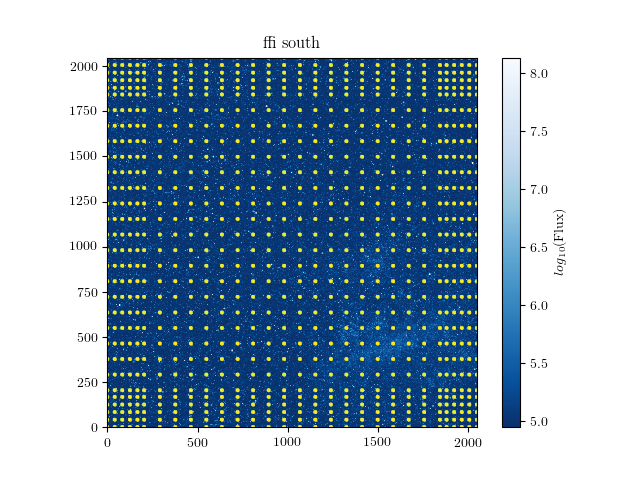
\includegraphics[width=\textwidth]{OH_example}
\caption{Example of the spread of measurement boxes across a TESS FFI.}
\label{fig:ojh}
\end{figure}


\subsection{RH estimate}
This method (method author: Rasmus Handberg) uses the \texttt{photutils} Background2d and SExtractorBackground packages. It first masks out any high flux values, then performs a 5-iteration sigma clip to 3 $\sigma$ before running the Background2D package using the SExtractorbackground as the background estimator. \\

Pros:
\begin{itemize}
\item Works quickly
\item The result is directly sampled from the data and not a featureless polynomial
\end{itemize}

Cons:
\begin{itemize}
\item Not certain how much of the small scale structure is reliable
\item Relies on some hard-coded parameters
\item Relies heavily on a single external module
\end{itemize}

\section{Test 1:  Flat Gaussian Noise Background}
To test the background estimators we first applied them to the most simple case: a FFI-shaped flat background with Gaussian noise. The noise was generated in a 2048x2048 Python meshgrid with a mean of 1000 and a standard deviation of 100. The resulting model can be seen in Figure \ref{fig:flatgauss}.\\

\begin{figure}[h!]
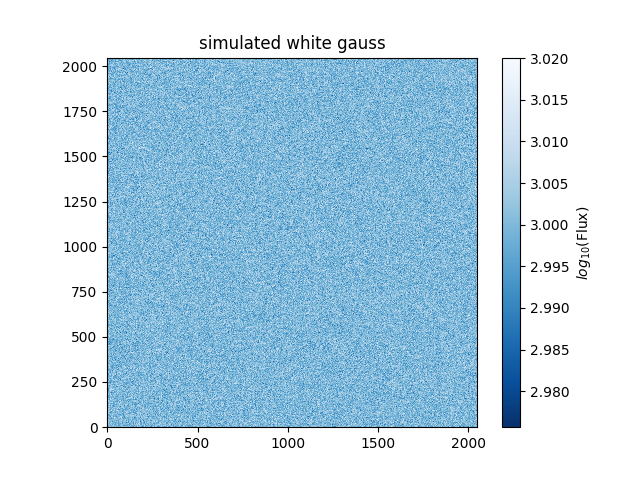
\includegraphics[width=\textwidth]{flatgauss}
\caption{Flat background of gaussian white noise}
\label{fig:flatgauss}
\end{figure}

The resulting distribution of estimated background points can be seen in Figure \ref{fig:histogram_flatgauss}. The residuals on the estimated background can be seen for every 2048th data point in Figure \ref{fig:residual_flatgauss}.

\begin{figure}[h!]
\centering
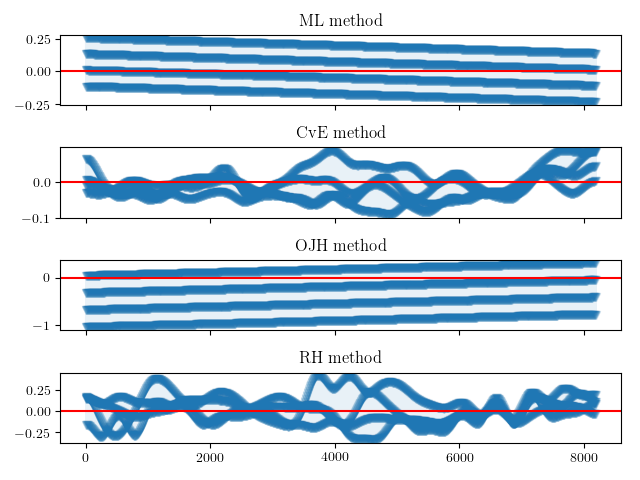
\includegraphics[width=0.49\textheight]{residual_flatgauss}
\caption{Every 2048th residual for the four different background estimators applied to a white noise background. The y-axis is residuals as a percentage of the background level. Note that only the residuals in one direction are shown, as it takes every 2048th data point}
\label{fig:residual_flatgauss}
\end{figure}

\begin{figure}[h!]
\centering
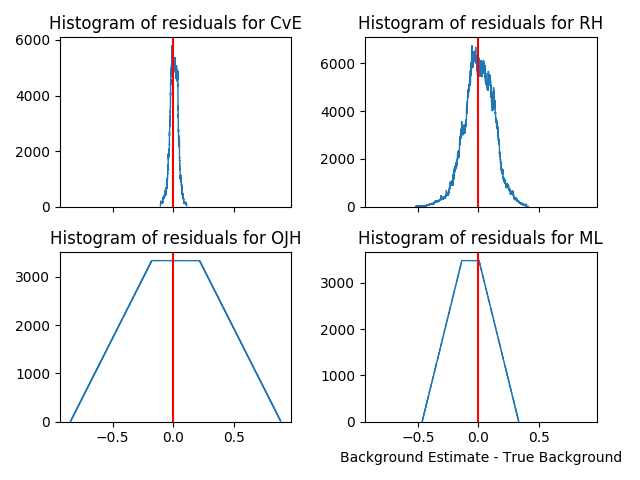
\includegraphics[width=0.49\textheight]{histogram_flatgauss}
\caption{Histograms of the residuals for the four different background estimators applied to a white noise background.}
\label{fig:histogram_flatgauss}
\end{figure}

\subsection{CvE}
The CvE method does not fare very well against this test unsupervised--- by default it measures the 10th percentile of the data, and when there are no high-flux stars contaminating each bin it will underestimate the background left unsupervised. However when setting the percentile to 50 it recovers the background to within 1$\sigma$ and thus performs well.\\

Changes made during this test:
\begin{itemize}
\item Now takes the x-th percentile in each bin where x is a default of 10, as opposed to the minimum.
\end{itemize}

\subsection{ML}
The ML method fares well against this test provided it is run with a low-order polynomial fit. Using a default first-order polynomial, the method comes within <1$\%$ of the background level, although it does find a slope that is not present in the data. The residuals center around 0, and thus the median of the background does yield the correct value.\\

Changes made during this test:
\begin{itemize}
\item The polynomial model now defaults to an order of 1.
\end{itemize}

\subsection{OJH}
The OJH method fares similarly to the MH method, where it finds a non-existent slope in its polynomial fit. In general, as can be seen from the histograms, it centers around the correct value.

Changes made during this test:
\begin{itemize}
\item The polynomial model now defaults to an order of 1.
\item The OJH method now also fits 500 iterations of RANSAC to the modes and uses the resulting inlier mask as weights on the polynomial fit in the same manner as the MH method. Without this addition, the background estimate was biased away from the true value.
\end{itemize}

\subsection{RH}
The RH method fares well on this test. No major changes had to be made.

Changes made during this test:
\begin{itemize}
\item The background estimation is now smoothed using a median filter before returning from the function.
\end{itemize}


\subsection{Conclusions}
In conclusion, all four methods are able to recover a distribution of residuals centered around 0., as would be expected for a simple background with no stars. All four backgrounds progress to the next stage of testing.

\begin{figure}[!ht]
   \centering
   \subfloat[][]{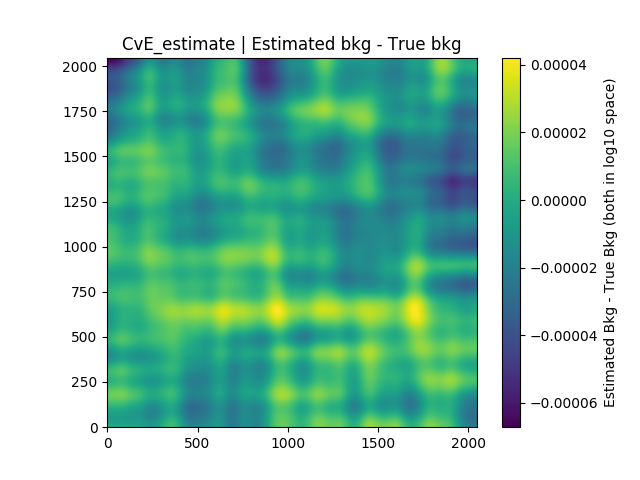
\includegraphics[width=.4\textwidth]{CvE_flatgauss}}\quad
   \subfloat[][]{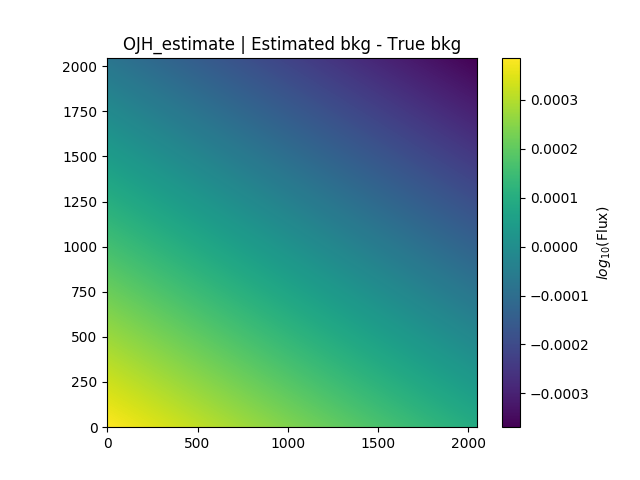
\includegraphics[width=.4\textwidth]{OH_flatgauss}}\\
   \subfloat[][]{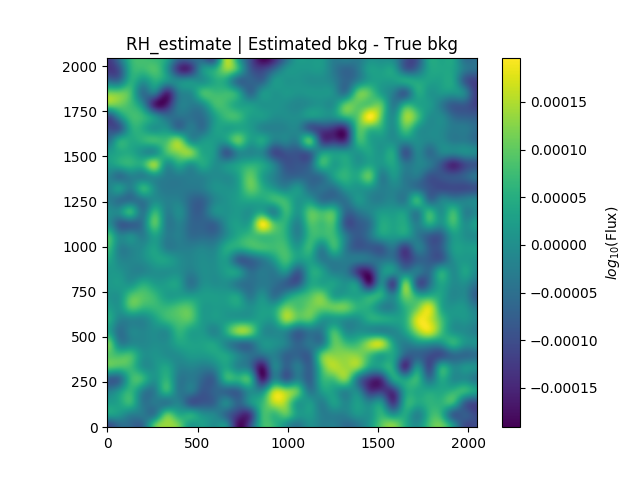
\includegraphics[width=.4\textwidth]{RH_flatgauss}}\quad
   \subfloat[][]{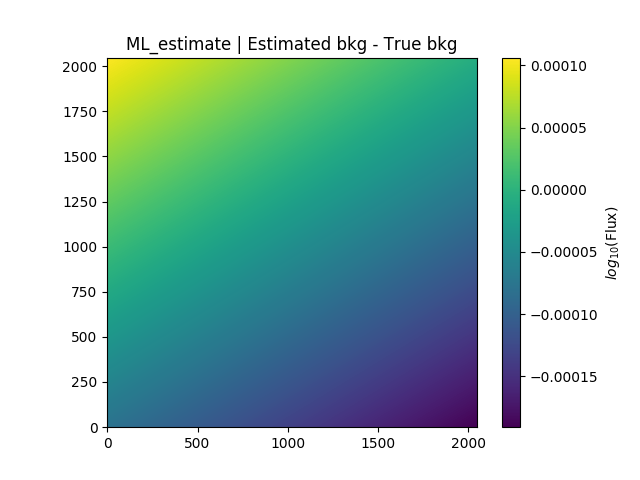
\includegraphics[width=.4\textwidth]{ML_flatgauss}}
   \caption{Residuals on background fits to a flat gaussian noise background.}
\end{figure}

\section{Test 2: Noise Background + slope and crowding}
The next stage of background estimator testing involves a more compliated background function. The background now consists of three components:

\begin{itemize}
\item A sloped background
\item A large area of increased background level in the shape of 2D Gaussian (to function as a crowded local area)
\item 2048 faint stars smoothed over before being added to the background (to function as unfocused stars)
\end{itemize}

The individual components, as well as the combined background and the simulated (star-less) FFI, can be seen in Figures \ref{fig:bkgcomponents} and \ref{fig:complexbkg}.

\begin{figure}
\centering
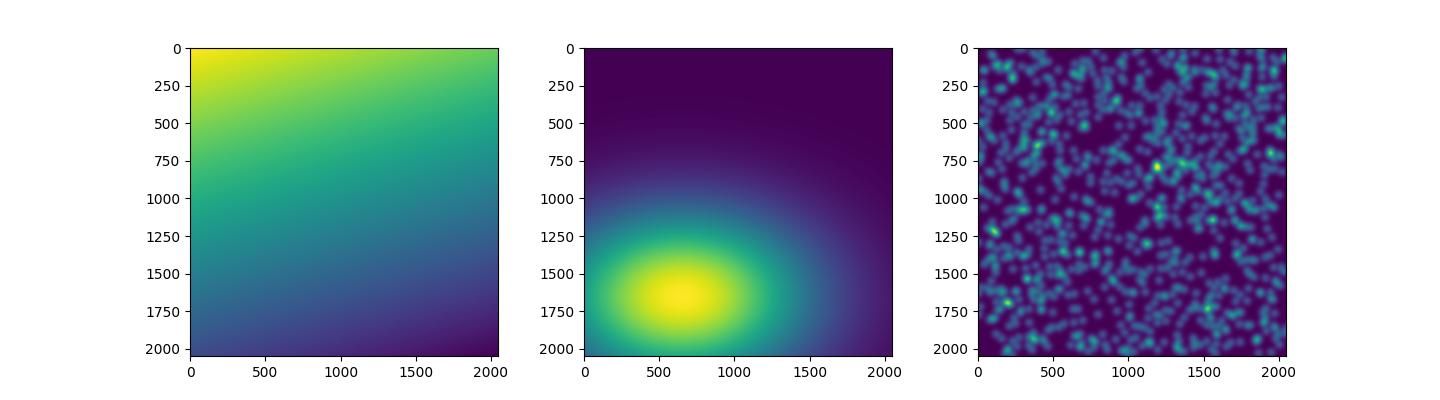
\includegraphics[width=\textwidth]{bkgcomponents}
\caption{The various components used in the new complex background.}
\label{fig:bkgcomponents}
\end{figure}


\begin{figure}[!ht]
   \centering
   \subfloat[][]{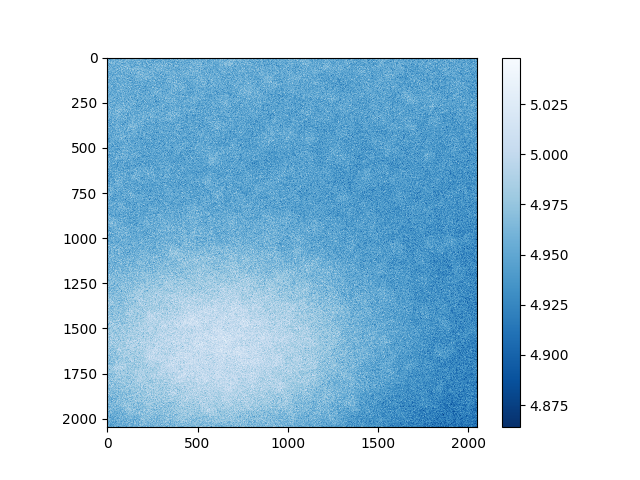
\includegraphics[width=.4\textwidth]{complexffi}}\quad
   \subfloat[][]{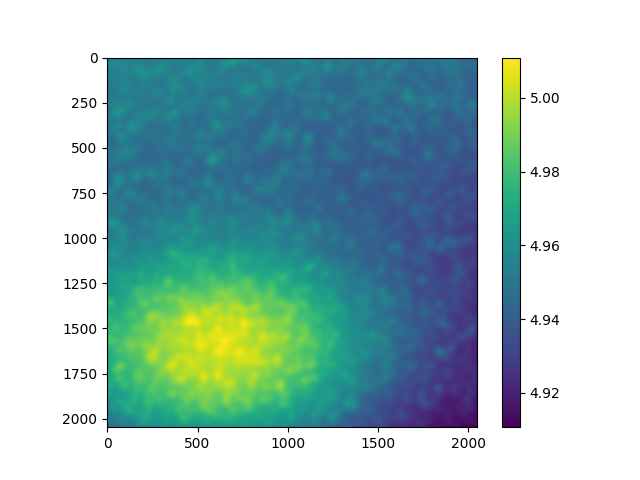
\includegraphics[width=.4\textwidth]{complexbkg}}\\
   \caption{Background without noise (for estimation evaluation) and with noise (on which the background is measured).
   \label{fig:complexbkg}
\end{figure}


\subsection{CvE}
\subsection{ML}
\subsection{OJH}
\subsection{RH}

\section{Test 3: The above + Stars}
\subsection{CvE}
\subsection{ML}
\subsection{OJH}
\subsection{RH}


\section{Conclusions}


\end{document}
